%!TEX TS-program = latex
\documentclass[landscape,final]{baposter}
\usepackage{amsmath,amssymb,amsfonts,amscd,amsthm}%-----amscd for "Commutative %Diagrams"

\usepackage{times}
\usepackage{calc}
\usepackage{graphicx, psfrag}
\usepackage{amsmath}
\usepackage{amssymb}
\usepackage{relsize}
\usepackage{multirow}
\usepackage{bm}

\usepackage{graphicx}
\usepackage{multicol}

\usepackage{pgfbaselayers}
\pgfdeclarelayer{background}
\pgfdeclarelayer{foreground}
\pgfsetlayers{background,main,foreground}

\usepackage{helvet}
%\usepackage{bookman}
\usepackage{palatino}

\newcommand{\captionfont}{\footnotesize}
\newtheorem{definition}{Definition}

\newtheorem{convention}{Convention}
\newtheorem{proposition}{Proposition}
\newtheorem{lemma}{Lemma}
\newtheorem{theorem}{Theorem}
\newtheorem{corollary}{Corollary}
\newtheorem{conjecture}{Conjecture}
\selectcolormodel{cmyk}

\graphicspath{{images/}}

%%%%%%%%%%%%%%%%%%%%%%%%%%%%%%%%%%%%%%%%%%%%%%%%%%%%%%%%%%%%%%%%%%%%%%%%%%%%%%%%
%%%% Some math symbols used in the text
%%%%%%%%%%%%%%%%%%%%%%%%%%%%%%%%%%%%%%%%%%%%%%%%%%%%%%%%%%%%%%%%%%%%%%%%%%%%%%%%
% Format 
\newcommand{\Matrix}[1]{\begin{bmatrix} #1 \end{bmatrix}}
\newcommand{\Vector}[1]{\Matrix{#1}}
\newcommand*{\SET}[1]  {\ensuremath{\mathcal{#1}}}
\newcommand*{\MAT}[1]  {\ensuremath{\mathbf{#1}}}
\newcommand*{\VEC}[1]  {\ensuremath{\bm{#1}}}
\newcommand*{\CONST}[1]{\ensuremath{\mathit{#1}}}
\newcommand*{\norm}[1]{\mathopen\| #1 \mathclose\|}% use instead of $\|x\|$
\newcommand*{\abs}[1]{\mathopen| #1 \mathclose|}% use instead of $\|x\|$
\newcommand*{\absLR}[1]{\left| #1 \right|}% use instead of $\|x\|$

\def\norm#1{\mathopen\| #1 \mathclose\|}% use instead of $\|x\|$
\newcommand{\normLR}[1]{\left\| #1 \right\|}% use instead of $\|x\|$

%%%%%%%%%%%%%%%%%%%%%%%%%%%%%%%%%%%%%%%%%%%%%%%%%%%%%%%%%%%%%%%%%%%%%%%%%%%%%%%%
% Multicol Settings
%%%%%%%%%%%%%%%%%%%%%%%%%%%%%%%%%%%%%%%%%%%%%%%%%%%%%%%%%%%%%%%%%%%%%%%%%%%%%%%%
\setlength{\columnsep}{0.7em}
\setlength{\columnseprule}{0mm}


%%%%%%%%%%%%%%%%%%%%%%%%%%%%%%%%%%%%%%%%%%%%%%%%%%%%%%%%%%%%%%%%%%%%%%%%%%%%%%%%
% Save space in lists. Use this after the opening of the list
%%%%%%%%%%%%%%%%%%%%%%%%%%%%%%%%%%%%%%%%%%%%%%%%%%%%%%%%%%%%%%%%%%%%%%%%%%%%%%%%
\newcommand{\compresslist}{%
\setlength{\itemsep}{1pt}%
\setlength{\parskip}{0pt}%
\setlength{\parsep}{0pt}%
}


%%%%%%%%%%%%%%%%%%%%%%%%%%%%%%%%%%%%%%%%%%%%%%%%%%%%%%%%%%%%%%%%%%%%%%%%%%%%%%
%%% Begin of Document
%%%%%%%%%%%%%%%%%%%%%%%%%%%%%%%%%%%%%%%%%%%%%%%%%%%%%%%%%%%%%%%%%%%%%%%%%%%%%%

\begin{document}

%%%%%%%%%%%%%%%%%%%%%%%%%%%%%%%%%%%%%%%%%%%%%%%%%%%%%%%%%%%%%%%%%%%%%%%%%%%%%%
%%% Here starts the poster
%%%---------------------------------------------------------------------------
%%% Format it to your taste with the options
%%%%%%%%%%%%%%%%%%%%%%%%%%%%%%%%%%%%%%%%%%%%%%%%%%%%%%%%%%%%%%%%%%%%%%%%%%%%%%
\typeout{Poster Starts}
\background{
  \begin{tikzpicture}[remember picture,overlay]%
    \draw (current page.north west)+(-2em,-0em) node[anchor=north west] {\hspace{-2em}\includegraphics[height=1.1\textheight]{silhouettes_background}};
  \end{tikzpicture}%
}
\definecolor{silver}{cmyk}{0,0,0,0.3}
\definecolor{yellow}{cmyk}{0,0,0.9,0.0}
\definecolor{reddishyellow}{cmyk}{0,0.22,1.0,0.0}
\definecolor{black}{cmyk}{0,0,0.0,1.0}
\definecolor{darkYellow}{cmyk}{0,0,1.0,0.5}
\definecolor{darkSilver}{cmyk}{0,0,0,0.1}

\definecolor{lightyellow}{cmyk}{0,0,0.3,0.0}
\definecolor{lighteryellow}{cmyk}{0,0,0.1,0.0}
\definecolor{lighteryellow}{cmyk}{0,0,0.1,0.0}
\definecolor{lightestyellow}{cmyk}{0,0,0.05,0.0}
\definecolor{gray}{cmyk}{0,0,0.0,0.6}

\begin{poster}{
  % Show grid to help with alignment
  grid=no,
  % Column spacing
  colspacing=1em,
  % Color style
  bgColorOne=white,
  bgColorTwo=lightestyellow,
  borderColor=gray,
  headerColorOne=darkSilver,
  headerColorTwo=reddishyellow,
  headerFontColor=black,
  boxColorOne=lightyellow,
  boxColorTwo=lighteryellow,
  % Format of textbox
  textborder=bars,
  % Format of text header
  eyecatcher=no,
  headerborder=open,
  headerheight=0.08\textheight,
  headershape=roundedright,
  headershade=plain,
  headerfont=\Large\textsf, %Sans Serif
  boxshade=plain,
%  background=shade-tb,
  background=plain,
  linewidth=2pt
  }
  % Eye Catcher
  {} % No eye catcher for this poster. If an eye catcher is present, the title is centered between eye-catcher and logo.
  % Title
  {\sf %Sans Serif
  %\bf% Serif
  Comet Tail Artifacts in Computed Tomography}
  % Authors
  {\sf %Sans Serif
  % Serif
  Ryan Hass \hspace{3em} Adel Faridani \hspace{3em}
  Oregon State University
  }
  % University logo
  {{\begin{minipage}{30em}
  	
	\begin{tabular}{cc}
    \includegraphics[height=4em]{osu_logo} &
    \includegraphics[height=4em]{nsfe.eps}
    \end{tabular}
  \end{minipage}}
  }

  \tikzstyle{light shaded}=[top color=baposterBGtwo!30!white,bottom color=baposterBGone!30!white,shading=axis,shading angle=30]

  % Width of left inset image
     \newlength{\leftimgwidth}
     \setlength{\leftimgwidth}{0.78em+8.0em}

%%%%%%%%%%%%%%%%%%%%%%%%%%%%%%%%%%%%%%%%%%%%%%%%%%%%%%%%%%%%%%%%%%%%%%%%%%%%%%
%%% Now define the boxes that make up the poster
%%%---------------------------------------------------------------------------
%%% Each box has a name and can be placed absolutely or relatively.
%%% The only inconvenience is that you can only specify a relative position 
%%% towards an already declared box. So if you have a box attached to the 
%%% bottom, one to the top and a third one which should be in between, you 
%%% have to specify the top and bottom boxes before you specify the middle 
%%% box.
%%%%%%%%%%%%%%%%%%%%%%%%%%%%%%%%%%%%%%%%%%%%%%%%%%%%%%%%%%%%%%%%%%%%%%%%%%%%%%
    %
    % A coloured circle useful as a bullet with an adjustably strong filling
    \newcommand{\colouredcircle}[1]{%
      \tikz{\useasboundingbox (-0.2em,-0.32em) rectangle(0.2em,0.32em); \draw[draw=black,fill=baposterBGone!80!black!#1!white,line width=0.03em] (0,0) circle(0.18em);}}

%%%%%%%%%%%%%%%%%%%%%%%%%%%%%%%%%%%%%%%%%%%%%%%%%%%%%%%%%%%%%%%%%%%%%%%%%%%%%%
  \headerbox{Contribution}{name=contribution,column=0,row=0}{
%%%%%%%%%%%%%%%%%%%%%%%%%%%%%%%%%%%%%%%%%%%%%%%%%%%%%%%%%%%%%%%%%%%%%%%%%%%%%%
   {}In computed tomography (CT) we recover a function $f$ from its x-ray data.  We model our x-ray data as line integrals of $f$ and then filter and backproject our data to recover $f$.  We present a study of artifacts that appear in a 3D reconstruction formula for CT \cite{kat} by studying the 2D case.
 }

%%%%%%%%%%%%%%%%%%%%%%%%%%%%%%%%%%%%%%%%%%%%%%%%%%%%%%%%%%%%%%%%%%%%%%%%%%%%%%
  \headerbox{Reconstruction Method}{name=model,column=0,below=contribution}{
%%%%%%%%%%%%%%%%%%%%%%%%%%%%%%%%%%%%%%%%%%%%%%%%%%%%%%%%%%%%%%%%%%%%%%%%%%%%%%
	We following the work of \cite{FHS}.  We have a rotating detector and x-ray source traveling around an object $f(x)$.  Here we assume a source curve $y(s) = (R \cos(s), R \sin(s))$ with radius $R$.  We have detector coordinates $e_u(s)$ and $e_v(s)$.  The vector $\Theta(s, x)$ points from $y(s)$ in the direction of $x$.  The angle between $e_u(s)$ and $\Theta(s, x)$ is $\alpha^*$.  The point $x$ has detector coordinate $\alpha^*$ and the x-ray data for $x$ is $g(s, \alpha^*)$.
	\begin{center}
		% This file is generated by the MATLAB m-file laprint.m. It can be included
% into LaTeX documents using the packages graphicx, color and psfrag.
% It is accompanied by a postscript file. A sample LaTeX file is:
%    \documentclass{article}\usepackage{graphicx,color,psfrag}
%    \begin{document}\input{TDwindow}\end{document}
% See http://www.mathworks.de/matlabcentral/fileexchange/loadFile.do?objectId=4638
% for recent versions of laprint.m.
%
% created by:           LaPrint version 3.16 (13.9.2004)
% created on:           23-Apr-2008 10:44:42
% eps bounding box:     15 cm x 11.25 cm
% comment:              
%

\begin{psfrags}%
\psfragscanon%
%
% text strings:
% \psfrag{x}[t][t]{\color[rgb]{0,0,0}\setlength{\tabcolsep}{0pt}\begin{tabular}{c}$x$ \end{tabular}}%

\psfrag{x}[t][t]{$x$}
\psfrag{y}[t][t]{$y(s)$}
\psfrag{a}[t][t]{$\alpha^*$}
\psfrag{u}[t][t]{$e_u(s)$}
\psfrag{v}[t][t]{$e_v(s)$}
\psfrag{t}[t][t]{$\Theta(s, x)$}
\psfrag{a}[t][t]{$\alpha^*$}
\psfrag{d}[t][t]{detector}

\psfrag{A}[t][t]{$g(s, \alpha^*)$}
%
% Figure:
\resizebox{3in}{!}{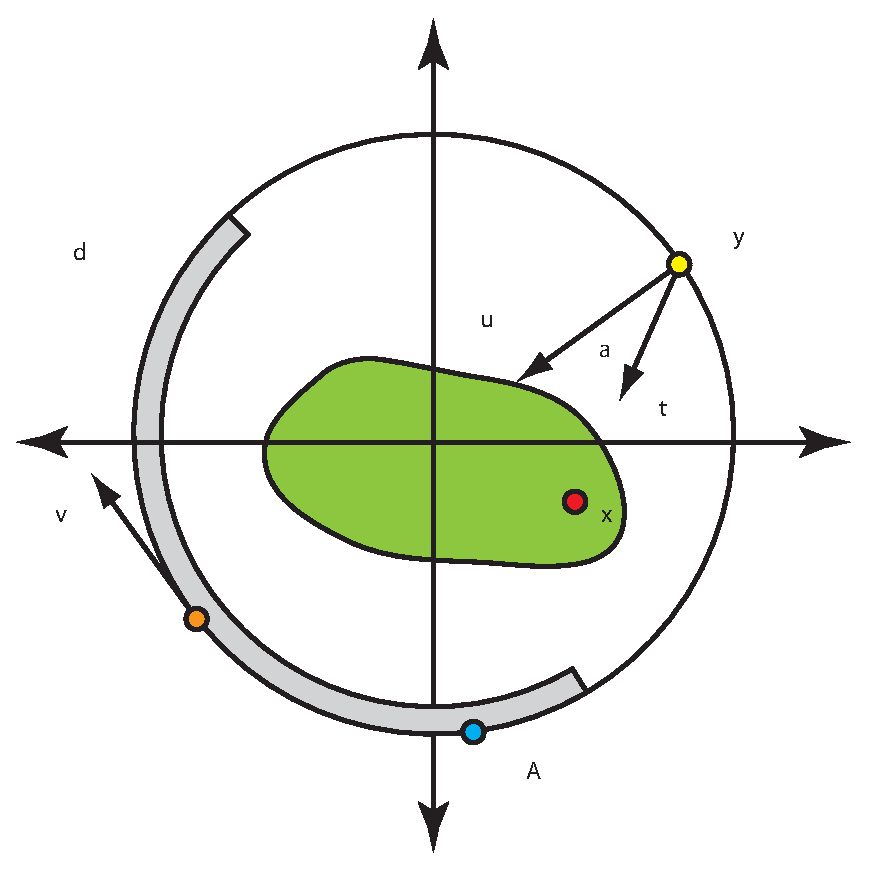
\includegraphics[width=.9\textwidth]{images/fanbeam_geometry.eps}}%
\end{psfrags}%
%
% End TDwindow.tex

	\end{center}
	We suppose that our x-ray data is given to us by\begin{equation}
	g(s, \alpha^*) = \int_0^{\infty}f(y(s) + t \Theta(s, x)) \; dt.
	\end{equation}
	Our formula for $f$ is a 2D analog of Katsevich's 3D formula,
	\begin{equation}
	\begin{split}
	f(x) & = \frac 1 {2 \pi^2} \int_{I_{PI}(x)} \frac 1 {|x - y(s)|} \\ & \quad \int_0^{2 \pi} 
		\Big ( \frac {\partial g} {\partial s} + \frac {\partial g} {\partial \alpha} \Big )
		\frac 1 {\sin(\alpha^{\star} - \alpha)} \; d\alpha \; ds
	\end{split}
	\end{equation}
   

  }


%%%%%%%%%%%%%%%%%%%%%%%%%%%%%%%%%%%%%%%%%%%%%%%%%%%%%%%%%%%%%%%%%%%%%%%%%%%%%%
  \headerbox{PI-lines}{name=results neutralization,column=1,row=0}{
%%%%%%%%%%%%%%%%%%%%%%%%%%%%%%%%%%%%%%%%%%%%%%%%%%%%%%%%%%%%%%%%%%%%%%%%%%%%%%
	\begin{definition}
	A PI-line is any line segment passing through $x$ that intersects the source curve at $y(s_b)$ and $y(s_t)$ such that $s_t - s_b \le 2 \pi$. 
	\end{definition}That is to say that $s_b$ and $s_t$ are separated by no more than one turn.  We call $I_{PI} (x) = [s_b, s_t]$ the Parametric Interval or the PI-interval of $x$.  In the 3D case with a helical source curve every point within the helix belongs to a unique PI-line.  This is not the case for a circle as there exists infinitely many such lines that intersect the scanning circle and contain $x$.

	For the 2D case we consider a few special families of PI-lines.  The first correspond to the PI-intervals from the Helix, modulo $2\pi$, for the points that lie in the plane $z = 0$.  \begin{multicols}{2}
	The second type of PI-lines considered are called orthogonal-long PI-lines.  We take a line through $x$ with slope perpendicular to the polar angle of $x$.  
	\begin{center}
	% This file is generated by the MATLAB m-file laprint.m. It can be included
% into LaTeX documents using the packages graphicx, color and psfrag.
% It is accompanied by a postscript file. A sample LaTeX file is:
%    \documentclass{article}\usepackage{graphicx,color,psfrag}
%    \begin{document}\input{TDwindow}\end{document}
% See http://www.mathworks.de/matlabcentral/fileexchange/loadFile.do?objectId=4638
% for recent versions of laprint.m.
%
% created by:           LaPrint version 3.16 (13.9.2004)
% created on:           23-Apr-2008 10:44:42
% eps bounding box:     15 cm x 11.25 cm
% comment:              
%

\begin{psfrags}%
\psfragscanon%
%
% text strings:
% \psfrag{x}[t][t]{\color[rgb]{0,0,0}\setlength{\tabcolsep}{0pt}\begin{tabular}{c}$x$ \end{tabular}}%

\psfrag{b}[t][t]{$s_b$}
\psfrag{t}[t][t]{$s_t$}
\psfrag{x}[t][t]{$x$}
\psfrag{a}[t][t]{$s_{b'}$}
\psfrag{u}[t][t]{$s_{t'}$}
\psfrag{A}[t][t]{$x'$}
%
% Figure:
\resizebox{2.7cm}{!}{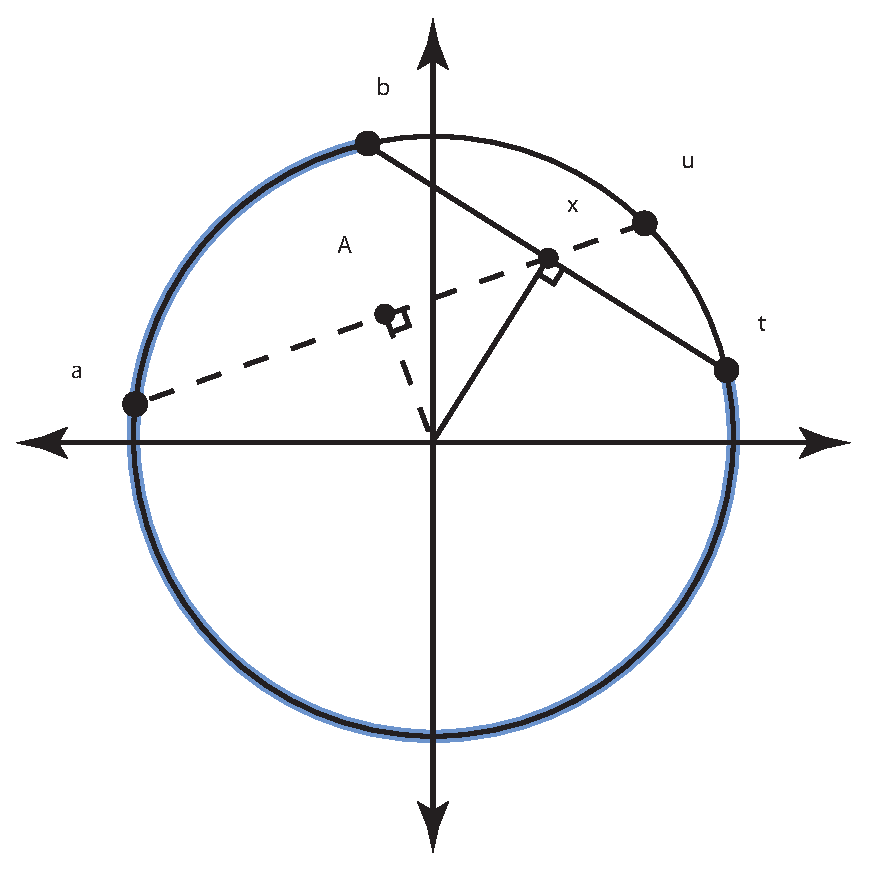
\includegraphics[width=0.4\textwidth]{images/orthogonal_pi_lines.eps}}%
\end{psfrags}%
%
% End TDwindow.tex

	\end{center}
	\end{multicols}
	
	The tilted-long PI-line of a point $x$ corresponds to a orthogonal PI-line for the point $x'$ where $x' = A x$ and $A$ is given by the matrix
	\begin{equation}
		A = \sin(\psi) \left [ 
		\begin{array}{cc} 
		\sin(\psi) & -\cos(\psi) \\  
		\cos(\psi) & \sin(\psi)
		\end{array}
		\right ].
\end{equation}
  }
%%%%%%%%%%%%%%%%%%%%%%%%%%%%%%%%%%%%%%%%%%%%%%%%%%%%%%%%%%%%%%%%%%%%%%%%%%%%%%
  \headerbox{Comet Tails}{name=robustness,column=1,below=results neutralization,span=1,above=bottom}{
%%%%%%%%%%%%%%%%%%%%%%%%%%%%%%%%%%%%%%%%%%%%%%%%%%%%%%%%%%%%%%%%%%%%%%%%%%%%%%
	Let $f(x)$ be a smooth compactly supported function.  Below are $f(x)$ and reconstructions of $f(x)$ by equation 1 with orthogonal-long and helical pi-lines.
	\begin{tabular}{ccc}
		& & \\
		\input{images/original} &
		\input{images/orthogonal-long} &
		% This file is generated by the MATLAB m-file laprint.m. It can be included
% into LaTeX documents using the packages graphicx, color and psfrag.
% It is accompanied by a postscript file. A sample LaTeX file is:
%    \documentclass{article}\usepackage{graphicx,color,psfrag}
%    \begin{document}% This file is generated by the MATLAB m-file laprint.m. It can be included
% into LaTeX documents using the packages graphicx, color and psfrag.
% It is accompanied by a postscript file. A sample LaTeX file is:
%    \documentclass{article}\usepackage{graphicx,color,psfrag}
%    \begin{document}% This file is generated by the MATLAB m-file laprint.m. It can be included
% into LaTeX documents using the packages graphicx, color and psfrag.
% It is accompanied by a postscript file. A sample LaTeX file is:
%    \documentclass{article}\usepackage{graphicx,color,psfrag}
%    \begin{document}\input{helical}\end{document}
% See http://www.mathworks.de/matlabcentral/fileexchange/loadFile.do?objectId=4638
% for recent versions of laprint.m.
%
% created by:           LaPrint version 3.16 (13.9.2004)
% created on:           06-Feb-2009 12:54:08
% eps bounding box:     15 cm x 12.3485 cm
% comment:              
%
\begin{psfrags}%
\psfragscanon%
%
% text strings:
\psfrag{s02}[b][b]{\color[rgb]{0,0,0}\setlength{\tabcolsep}{0pt}\begin{tabular}{c}helical\end{tabular}}%
%
% xticklabels:
\psfrag{x01}[t][t]{50}%
\psfrag{x02}[t][t]{100}%
\psfrag{x03}[t][t]{150}%
\psfrag{x04}[t][t]{200}%
\psfrag{x05}[t][t]{250}%
%
% yticklabels:
\psfrag{v01}[r][r]{50}%
\psfrag{v02}[r][r]{100}%
\psfrag{v03}[r][r]{150}%
\psfrag{v04}[r][r]{200}%
\psfrag{v05}[r][r]{250}%
%
% Figure:
\resizebox{2.25cm}{!}{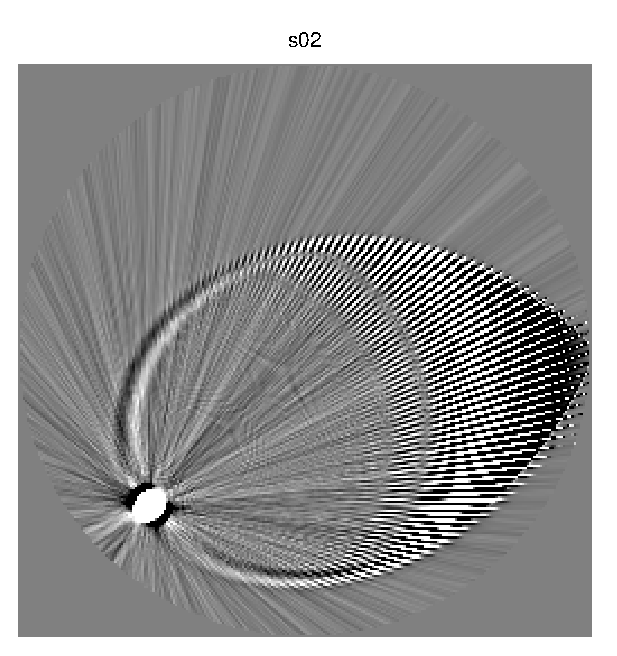
\includegraphics[width=0.4\textwidth]{images/helical.eps}}%
\end{psfrags}%
%
% End helical.tex
\end{document}
% See http://www.mathworks.de/matlabcentral/fileexchange/loadFile.do?objectId=4638
% for recent versions of laprint.m.
%
% created by:           LaPrint version 3.16 (13.9.2004)
% created on:           06-Feb-2009 12:54:08
% eps bounding box:     15 cm x 12.3485 cm
% comment:              
%
\begin{psfrags}%
\psfragscanon%
%
% text strings:
\psfrag{s02}[b][b]{\color[rgb]{0,0,0}\setlength{\tabcolsep}{0pt}\begin{tabular}{c}helical\end{tabular}}%
%
% xticklabels:
\psfrag{x01}[t][t]{50}%
\psfrag{x02}[t][t]{100}%
\psfrag{x03}[t][t]{150}%
\psfrag{x04}[t][t]{200}%
\psfrag{x05}[t][t]{250}%
%
% yticklabels:
\psfrag{v01}[r][r]{50}%
\psfrag{v02}[r][r]{100}%
\psfrag{v03}[r][r]{150}%
\psfrag{v04}[r][r]{200}%
\psfrag{v05}[r][r]{250}%
%
% Figure:
\resizebox{2.25cm}{!}{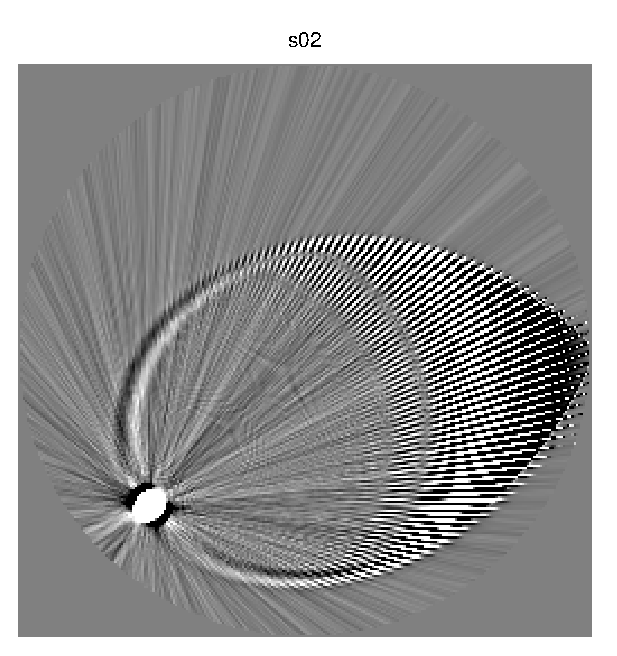
\includegraphics[width=0.4\textwidth]{images/helical.eps}}%
\end{psfrags}%
%
% End helical.tex
\end{document}
% See http://www.mathworks.de/matlabcentral/fileexchange/loadFile.do?objectId=4638
% for recent versions of laprint.m.
%
% created by:           LaPrint version 3.16 (13.9.2004)
% created on:           06-Feb-2009 12:54:08
% eps bounding box:     15 cm x 12.3485 cm
% comment:              
%
\begin{psfrags}%
\psfragscanon%
%
% text strings:
\psfrag{s02}[b][b]{\color[rgb]{0,0,0}\setlength{\tabcolsep}{0pt}\begin{tabular}{c}helical\end{tabular}}%
%
% xticklabels:
\psfrag{x01}[t][t]{50}%
\psfrag{x02}[t][t]{100}%
\psfrag{x03}[t][t]{150}%
\psfrag{x04}[t][t]{200}%
\psfrag{x05}[t][t]{250}%
%
% yticklabels:
\psfrag{v01}[r][r]{50}%
\psfrag{v02}[r][r]{100}%
\psfrag{v03}[r][r]{150}%
\psfrag{v04}[r][r]{200}%
\psfrag{v05}[r][r]{250}%
%
% Figure:
\resizebox{2.25cm}{!}{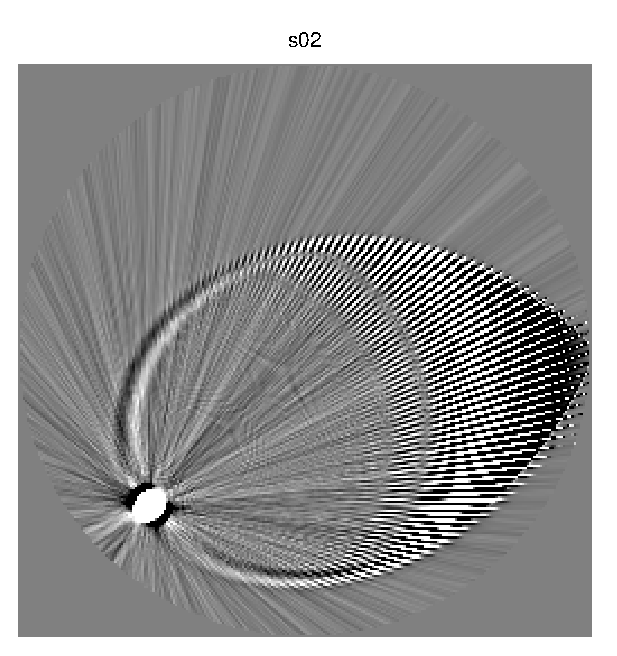
\includegraphics[width=0.4\textwidth]{images/helical.eps}}%
\end{psfrags}%
%
% End helical.tex

	\end{tabular}
	The long tail coming off of the function is called a comet tail artifact.  The artifact also occurs in reconstructions from the 3D version of formula 1, however with a much stronger presence.
  }
%%%%%%%%%%%%%%%%%%%%%%%%%%%%%%%%%%%%%%%%%%%%%%%%%%%%%%%%%%%%%%%%%%%%%%%%%%%%%%
  \headerbox{Results}{name=results,column=2,span=2,row=0}{
%%%%%%%%%%%%%%%%%%%%%%%%%%%%%%%%%%%%%%%%%%%%%%%%%%%%%%%%%%%%%%%%%%%%%%%%%%%%%%
\begin{multicols}{2}
	\begin{definition}
		We call $RBP(s) = \{x : s \in I_{PI}(x) \}$ the region of back projection associated with position $y(s)$. 
	\end{definition}
The shape of the region of back projection in the 2D plane is directly related to the behavior of the comet tail artifact found in the 2D Katsevich algorithm.  We will now describe the region of back projection for orthogonal and tilted PI-lines.
Let $B$ be the unit ball in $\mathbb{R}^2$.
\begin{theorem}
Suppose $R = 1$ and let $s \in [0, 2 \pi)$, then for the PI-lines of the orthogonal-long type we have $RBP(s) = B \cap D(s)$ where $D(s) = \{x : \|x - c \|_{2} \ge 1 / 2\}$ and $c = (\cos(s) / 2, \sin(s) / 2)$.
\end{theorem}
The $RBP(s)$ for the tilted-long PI-lines follows immediately.
\begin{corollary}
Suppose $R = 1$ and consider $B$ with the PI-lines of the tilted-long type.  Let $s \in [0, 2 \pi)$, then $s \in I_{PI}(x)$, for all $x \in B \cap D(s)$ where $D(s) = \{x : \|x - A^{-1}c \|_{2} \ge \frac 1 {2 \sin(\psi)} \}$ and $c = (\cos(s) / 2, \sin(s) / 2)$.
\end{corollary}
\begin{proof}(Outline)
This follows from Theorem 1 and the fact that
\begin{eqnarray*}
	\frac 1 4 & \le & \langle Ax - c, Ax - c \rangle \\
	& = & \langle Ax - A A^{-1}c, Ax - c \rangle \\
	& = & \langle x - A^{-1}c, A^* Ax - A^* c \rangle \\
	& = & \langle x - A^{-1}c, \sin^{2}(\psi) x - \sin^{2}(\psi)A^{-1} c \rangle \\
	& = & \sin^2 (\psi) \langle x - A^{-1}c, x - A^{-1}c \rangle.
\end{eqnarray*}
Hence $\| Ax - c \|_{2} \ge \frac 1 2$ if and only if $\| x - A^{-1}c \|_{2} \ge \frac 1 {2 \sin (\psi)}$.
\end{proof}

We can now identify where along the boundary of $RBP(s)$ a point $x$ will backproject to.  This corresponds to the end points of the outer integral in equation 1.

\begin{theorem}
\label{artifact_shape}
Let $f(x)$ be a delta function located at $(x_0, y_0) \in B$.  Let $\gamma(s)$ be the point on the boundary of $RBP(s)$ connecting $(x_0, y_0)$ to $y(s)$.  Then for the PI-lines of the orthogonal-long type we have $\gamma(s) = \frac d 2 (\cos(s + k), \sin(s + k)) + (\frac {x_0} 2, \frac {y_0}  2)$, for $d = \sqrt{x_0^2 + y_0^2}$, $k$ is a constant.
\end{theorem}
\begin{proof}(Outline)
We will use geometric argument that follows from the following diagram.
	\begin{center}
		% This file is generated by the MATLAB m-file laprint.m. It can be included
% into LaTeX documents using the packages graphicx, color and psfrag.
% It is accompanied by a postscript file. A sample LaTeX file is:
%    \documentclass{article}\usepackage{graphicx,color,psfrag}
%    \begin{document}\input{TDwindow}\end{document}
% See http://www.mathworks.de/matlabcentral/fileexchange/loadFile.do?objectId=4638
% for recent versions of laprint.m.
%
% created by:           LaPrint version 3.16 (13.9.2004)
% created on:           23-Apr-2008 10:44:42
% eps bounding box:     15 cm x 11.25 cm
% comment:              
%

\begin{psfrags}%
\psfragscanon%
%
% text strings:
% \psfrag{x}[t][t]{\color[rgb]{0,0,0}\setlength{\tabcolsep}{0pt}\begin{tabular}{c}$x$ \end{tabular}}%

\psfrag{A}[t][t]{$A$}
\psfrag{B}[t][t]{$B$}
\psfrag{C}[t][t]{$C$}
\psfrag{D}[t][t]{$D$}
\psfrag{E}[t][t]{$E$}
\psfrag{F}[t][t]{$F$}
\psfrag{a}[t][t]{$\alpha$}
%
% Figure:
\resizebox{1.5in}{!}{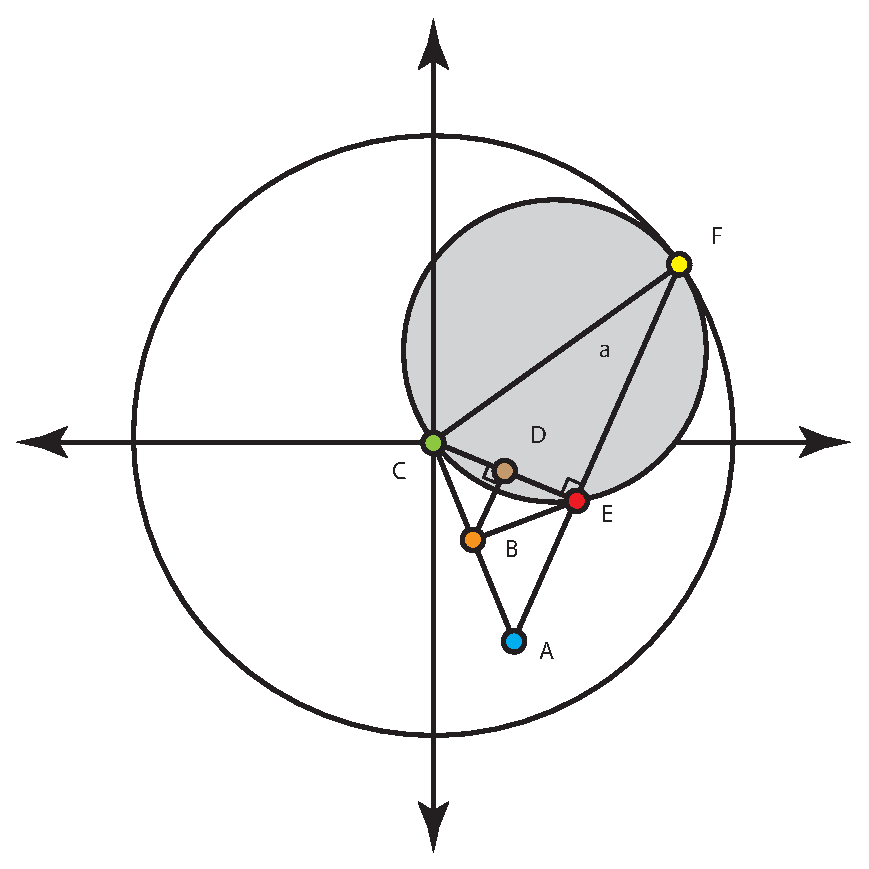
\includegraphics[width=0.3\textwidth]{images/artifact_circle_argument.eps}}%
\end{psfrags}%
%
% End TDwindow.tex

	\end{center}
Let $A = (x_0, y_0), B = (\frac {x_0} {2}, \frac {y_0} {2}), C = (0, 0)$, and $F = y(s)$.  Let $B$ be the midpoint between $A$ and $C$ and let $D$ be the midpoint between $C$ and $E$.  Let $E = \gamma(s)$.  We will show the distance from $E$ to $B$ is fixed for all source positions.

The line segment $CE$ is perpendicular to line segment $AF$ since $E$ lies on a circle in the middle of $C$ and $F$.  Therefore triangle $ACE$ is similar to triangle $BCD$.  Furthermore triangle $BCD$ is congruent to triangle $BED$.  In particular we have that line segments $BA$, $BC$ and $BE$ have the same length.  Since $BC$ has fixed length we can conclude that the path of $\gamma(s)$ is a circle centered at $B$.
\end{proof}

It is difficult to analytically describe the region of back projection for the helical PI-lines.  The study of the orthogonal-long PI-lines has validated that the source of the comet tail artifact is the endpoints of integration in equation 1, $I_{PI}(x)$.

      \end{multicols}\vspace{-1em}
  }%
%%%%%%%%%%%%%%%%%%%%%%%%%%%%%%%%%%%%%%%%%%%%%%%%%%%%%%%%%%%%%%%%%%%%%%%%%%%%%%
  \headerbox{Closing Remarks}{name=remarks,column=2,span=1,above=bottom,below=results}{
%%%%%%%%%%%%%%%%%%%%%%%%%%%%%%%%%%%%%%%%%%%%%%%%%%%%%%%%%%%%%%%%%%%%%%%%%%%%%%
    We have shown that the selection of PI-lines will effect the shape of the RBP(s).  Furthermore we have created a method to determine where along the boundary of RBP(s) x-ray data from a point source will backproject to.  The curve $\gamma(s)$ in Theorem 2 corresponds to the location of the comet tail artifact associated with orthogonal-long pi-lines.
  }%
%%%%%%%%%%%%%%%%%%%%%%%%%%%%%%%%%%%%%%%%%%%%%%%%%%%%%%%%%%%%%%%%%%%%%%%%%%%%%%
  \headerbox{Funding}{name=funding,column=3,span=1,above=bottom}{
%%%%%%%%%%%%%%%%%%%%%%%%%%%%%%%%%%%%%%%%%%%%%%%%%%%%%%%%%%%%%%%%%%%%%%%%%%%%%%
  \smaller 
  This work was supported in part by NSF grant DMS-0709495.
  }%
%%%%%%%%%%%%%%%%%%%%%%%%%%%%%%%%%%%%%%%%%%%%%%%%%%%%%%%%%%%%%%%%%%%%%%%%%%%%%%
  \headerbox{References}{name=references,column=3,above=funding,below=results}{
%%%%%%%%%%%%%%%%%%%%%%%%%%%%%%%%%%%%%%%%%%%%%%%%%%%%%%%%%%%%%%%%%%%%%%%%%%%%%%
    \smaller
\vspace{-0.4em}
    \bibliographystyle{acm}
    \renewcommand{\section}[2]{\vskip 0.05em}
      \begin{thebibliography}{1}\itemsep=-0.01em
      \setlength{\baselineskip}{0.4em}
      \bibitem{FHS}
        A.~Faridani, R.~Hass, D. Solmon.
        \newblock Numerical and theoretical explorations in helical and fan-beam tomography
        \newblock In {\em Journal of Physics: Conference Series, 2008}
      \bibitem{kat}
		A. Katsevich.
        \newblock Theoretically Exact Filtered Backprojection-Type Inversion Algorithm for Spiral CT
        \newblock In {\em SIAM Journal on Applied Mathematics, 2002}
      \end{thebibliography}
  }%
\end{poster}%
%
\end{document}
